L'objet de ce TP est de travailler avec des objets énumérables et des boucles d'énumération en manipulant un dessin ASCII qui remonte aux débuts de l'informatique\footnote{programmes cowsay et cowthink}. L'intruction \texttt{range} n'est autorisée que dans la dernière question.
\begin{enumerate}
 \item Sur votre fichier source dans votre éditeur, reproduisez le code suivant qui nomme une certaine chaine de caractères.
\begin{verbatim}
Vache = '''
  
   ^__^             
   (oo)\_______     
   (__)\       )\/\ 
       ||----w |    
       ||     ||    
  
'''
\end{verbatim}
Le dos, le haut et le bas de la tête sont formés avec des underscores (trait du 8). Les autres caractères sont faciles à deviner. Attention s'il y a plusieurs touches pour le slash / sur votre clavier, utiliser toujours la même.\newline 
On remarquera que le triple apostrophe \texttt{' ' '} ou \texttt{"""} est un délimiteur valide pour une construction littérale de chaine de caractères s'étendant sur plusieurs lignes.\footnote{Il n'est donc pas tout à fait correct de le considérer comme un commentaire mais plutôt comme une chaine anonyme qui sera donc \og oubliée\fg par l'interpréteur car elle n'a pas de nom.}\newline
Faire afficher le dessin par le script avec la commande \texttt{print} et faites exécuter votre script pour vérification. Réglez les paramètres de l'exécution pour vous permettre d'interagir avec l'interpréteur. Comparer le résultat du\texttt{print} avec l'entrée de \texttt{Vache} dans l'interpréteur. Comme le backslash \ joue un rôle particulier pour l'interpréteur (échappement), il est doublé dans la chaine de caractères. 
\item Au début de l'informatique les chaines de caractères n'étaient formées qu'à partir de 128 caractères (code ASCII). On peut en utiliser des milliers maintenant, ils sont codés dans des alphabets binaire ou octal ou hexadécimal mais ils sont aussi numérotés. Si \texttt{c} désigne un caractère (unicode)la commande \texttt{ord(c)} renvoie son numéro qui est un entier.  Inversement pour un entier \texttt{n}, la commande \texttt{chr(n)} renvoie le caractère de numéro \texttt{n}.
\begin{enumerate}
 \item Quels sont les caractères de numéros 47, 60, 92, 95, 8254, 8725 ?
 \item En utilisant \texttt{lili.append(truc)} pour insérer \texttt{truc} à la fin de la liste \texttt{lili} ainsi que \texttt{in} dans un test, former la liste de tous les numéros distincts des caractères qui forment \texttt{Vache}. En examinant la suite des caractères de \texttt{Vache}, Que pensez vous de celui de numéro 10? Est-il égal à la chaine de caractère \verb|'\n'|?
\end{enumerate}
\item Dans cette question, on utilisera la méthode \texttt{replace}. Si \texttt{chacha} est le nom d'une chaine de caractères, l'appel \texttt{chacha.replace('machin','truc')} renvoie une chaine de caractère formée à partir de \texttt{chacha} en replaçant chaque ocurrence de la chaine \texttt{'machin'} par la chaine \texttt{'truc'}. Attention, une chaine est non mutable donc il faut absolument assigner le résultat.
\begin{enumerate}
 \item En utilisant une boucle d'énumération, former à partir de \texttt{Vache} une nouvelle chaine de caractères permettant d'afficher
\begin{verbatim}
  
             ^__^   
     _______/(oo)   
 /\/(       /(__)   
    | w----||       
    ||     ||       
   
\end{verbatim}
\item Former de même une nouvelle chaine permettant d'afficher la vache la tête en bas. 
\end{enumerate}
\item Dans cette question on utilisera la méthode \texttt{splitlines}.\newline L'appel \texttt{chacha.splitlines()} renvoie la liste des lignes composant \texttt{chacha} (séparées par les caractères \verb|'\n'|). Afficher les trois vaches côte à côte.
\begin{figure}[h]
 \centering
 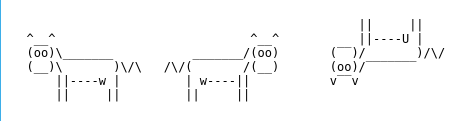
\includegraphics{./Evachscii_1.png}
 % Evachscii_1.png: 0x0 pixel, 0dpi, 0.00x0.00 cm, bb=
\end{figure}

\end{enumerate}
